\documentclass{article}
\usepackage{graphicx}

\graphicspath{{./img/}}
\title{2411 Project 3}
\author{Duncan Wilkie}
\date{1 October 2021}

\begin{document}

\maketitle

\section{}
\subsection{Analytical Solution}
The antiderivative of $e^{-t}$ is $-e^{-t}$. Evaluating this at the bounds yields a result of $-e^{-1} - (-1)=1-e^{-1}=0.632120558829$.
\subsection{Numerical Method}
We may use the three integration techniques learned so far to approximate this integral. We implement these in $C++$, and compare their perfomance.
\subsection{Program 1 Analysis}
The code written for this section, which implements the trapezoid and Simpson's rule, appears in the Script Files part. A log-log plot of the relative errors of each method as a function of the number of points used appears below.
\[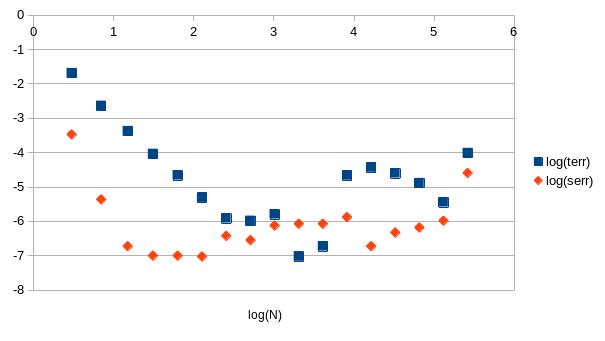
\includegraphics[scale=0.5]{plot1.png}\]
The convergence behavior exhibits significant difference: Simpson's rule converges by roughly $N=34$, whereas it takes the trapezoid rule until roughly $N=255$ for its error to settle near its final value.
Both methods acheive similar minimums of their error, near the machine precision at $10^{-7}$ in each case. However, Simpson's rule acheives it sooner, and its error stays lower for longer, compared to the trapezoid rule whose error increases to around $10^{-4}$ at the end of the $N$ interval considered.
Simpson's rule has a smaller approximation error for fixed $N$, both in theory and evidenced by this plot, as the trapezoid rule has $O(1/N^2)$ behavior and Simpson's has $O(1/N^4)$ behavior.
The total computational error for the trapezoid rule is $\frac{1}{N^2}+10^{-8}\sqrt{N}$ which is minimized when its derivative is zero, i.e. at \[\frac{-2}{N^3}+\frac{10^{-8}}{2\sqrt{N}}=0\Leftrightarrow N=(2\times 10^8)^{2/5}=2091\]
The total computational error for Simpson's rule is $\frac{1}{N^4}+10^{-8}\sqrt{N}$ which is minimized when its derivative is zero, i.e. at \[\frac{-4}{N^5}+\frac{10^{-8}}{2\sqrt{N}}=0\Leftrightarrow N=(4\times 10^8)^{2/9}=60\]
\subsection{TSG Program Analysis}
The program written for this section appears in the Script Files. The resulting log-log plot of the absolute errors in each method as a function of $N$ from 3 to 502 appears below.
\[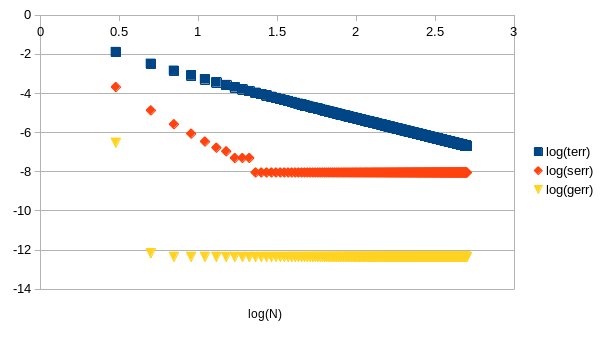
\includegraphics[scale=0.5]{plot2.png}\]
The Gauss rule converges much faster than the other two, taking only around three points to approach machine precision.

\section{}
The program written for this section appears in the Script Files. The resulting log-log plot of the absolute errors in each method as a function of $N$ appears below.
\[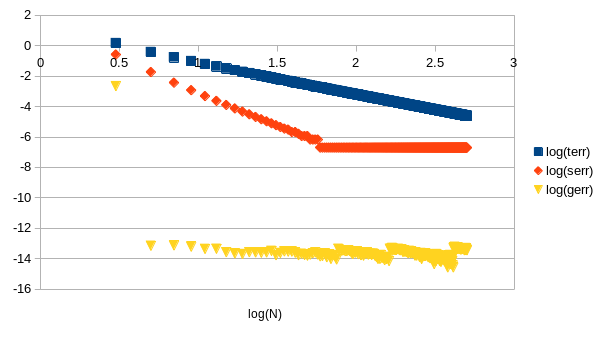
\includegraphics[scale=0.5]{plot3.png}\]
Only five points are needed to eliminate approximation error, as Gauss's rule is exact for polynomials of degree $2N-1$ and this polynomial is degree 8.
\section{}
The program written for this section appears in the Script Files. The resulting log-log plot of the absolute errors in each method as a function of $N$ appears below.
\[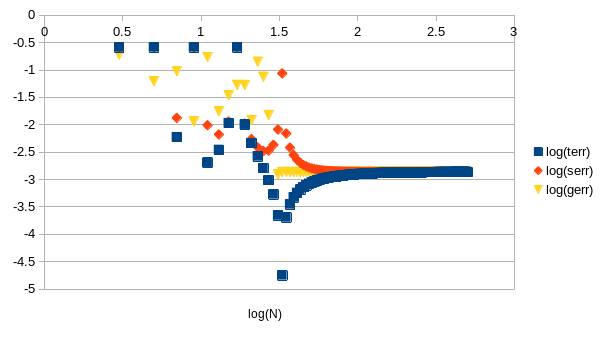
\includegraphics[scale=0.5]{plot4.png}\]
The trapezoid rule appears to do the best for most $N$. 
\section*{Script Files}
\subsection{Program 1}
\begin{verbatim}
Script started, file is dwilk14_proj3p1.txt
[dwilk14@tigers ~/Project3]$ cat dwilk14_proj3p1.cpp
#include <fstream>
#include <iostream>
#include <cmath>

using namespace std;

float simpson(float (*f)(float), float a, float b, int n) {
  float x, delta = (b - a) / (n - 1);
  
  float total = 0;

  for (int i = 1; i < n - 1; i += 2) { // odd
    x = a + i * delta;
    total += 4 * f(x);
  }

  for (int i = 2; i < n - 2; i += 2) { // even
    x = a + i * delta;
    total += 2 * f(x);
  }

  total += f(a) + f(b);
  total *= delta / 3;

  return total;
  
}

float trapezoid(float (*f)(float), float a, float b, int n) {
  float delta = (b - a) / (n - 1);
  float x = a;

  float total = 0;
  for (int i = 1; i < n - 1; i++) {
    x +=  delta;
    total += f(x);
  }

  total += (f(b) + f(a)) / 2;
  total *= delta;
  
  return total;
  
}

float nexp(float x) {
  return exp(-x);
}

int main() {
  int n = 3;
  float exact = 0.632120558829;
  ofstream ofile;
  ofile.open("output.txt");

  ofile << "n\tT err\tS err" << endl;

  while (n < 500000) {
    ofile << n << " " << abs(trapezoid(nexp, 0.0, 1.0, n) - exact) / exact \
          << " " << abs(simpson(nexp, 0.0, 1.0, n) - exact) / exact << endl;
    n = n * 2 + 1;
  }


  return 0;

}
[dwilk14@tigers ~/Project3]$ g++ dwilk14_proj3p1.cpp -o dwilk14_proj3p1
[dwilk14@tigers ~/Project3]$ ./dwilk14_proj3p1
[dwilk14@tigers ~/Project3]$ cp dwilk14_proj3p1.txt /home3/kristina/phys2411/.
[dwilk14@tigers ~/Project3]$ exit
exit
Script done, file is dwilk14_proj3p1.txt
\end{verbatim}
\subsection{TSG Program}
\begin{verbatim}
Script started, file is dwilk14_proj3p2.txt
[dwilk14@tigers ~/Project3]$ cat integTSG.cpp
#include <fstream>
#include <iostream>
#include <cmath>
#include "gauss.cpp"

using namespace std;

float simpson(double (*f)(double), double a, double b, int n) {
  double x, delta = (b - a) / (n - 1);
  
  double total = 0;

  for (int i = 1; i < n - 1; i += 2) { // odd
    x = a + i * delta;
    total += 4 * f(x);
  }

  for (int i = 2; i < n - 2; i += 2) { // even
    x = a + i * delta;
    total += 2 * f(x);
  }

  total += f(a) + f(b);
  total *= delta / 3;

  return total;
  
}

double trapezoid(double (*f)(double), double a, double b, int n) {
  double delta = (b - a) / (n - 1);
  double x = a;

  double total = 0;
  for (int i = 1; i < n - 1; i++) {
    x +=  delta;
    total += f(x);
  }

  total += (f(b) + f(a)) / 2;
  total *= delta;
  
  return total;
  
}

double gauss_integr (double (*f)(double), double min, double max,  int no) {                  // Gauss' rule
  int n;
  double quadra= 0.;
  double w[1000], x[1000];
  void gauss(int npts,int job,double a,double b,double x[],double w[]);         // for points and weights

  gauss (no, 0, min, max, x, w);                            // Gauss Legendre points & wts
  for (n = 0; n< no; n++) quadra += f(x[n])*w[n];                  // Calc integral
  return (quadra);
}


double nexp(double x) {
  return exp(-x);
}

int main() {
  ofstream outfile;
  outfile.open("output2.txt");
  double exact = 0.632120558829, a = 1, b = 2, step = (b - a) / 100;

  outfile << "n Terr Serr Gerr" << endl;
 
  for(int n = 3; n < 502; n += 2) {
    outfile << n << " " << abs(trapezoid(nexp, 0, 1, n)-exact) << " "
         << abs(simpson(nexp, 0, 1, n)-exact)
         << " " <<  abs(gauss_integr(nexp, 0, 1, n) - exact) << endl;
  }

  return 0;

}
[dwilk14@tigers ~/Project3]$ g++ integTSG.cpp -o integTSG                                              [dwilk14@tigers ~/Project3]$ ./integTSG
[dwilk14@tigers ~/Project3]$ cp dwilk14_proj3p2.txt /home3/kristina/phys2411/.
[dwilk14@tigers ~/Project3]$ exit
exit
Script done, file is dwilk14_proj3p2.txt
\end{verbatim}
\subsection{Program 2}
\begin{verbatim}
Script started, file is dwilk14_proj3p3.txt
[dwilk14@tigers ~/Project3]$ cat dwilk14_proj3p2.cpp
#include <fstream>
#include <iostream>
#include <cmath>
#include "gauss.cpp"

using namespace std;

float simpson(double (*f)(double), double a, double b, int n) {
  double x, delta = (b - a) / (n - 1);
  
  double total = 0;

  for (int i = 1; i < n - 1; i += 2) { // odd
    x = a + i * delta;
    total += 4 * f(x);
  }

  for (int i = 2; i < n - 2; i += 2) { // even
    x = a + i * delta;
    total += 2 * f(x);
  }

  total += f(a) + f(b);
  total *= delta / 3;

  return total;
  
}

double trapezoid(double (*f)(double), double a, double b, int n) {
  double delta = (b - a) / (n - 1);
  double x = a;

  double total = 0;
  for (int i = 1; i < n - 1; i++) {
    x +=  delta;
    total += f(x);
  }

  total += (f(b) + f(a)) / 2;
  total *= delta;
  
  return total;
  
}

double gauss_integr (double (*f)(double), double min, double max,  int no) {                  // Gauss' rule
  int n;
  double quadra= 0.;
  double w[1000], x[1000];
  void gauss(int npts,int job,double a,double b,double x[],double w[]);         // for points and weights

  gauss (no, 0, min, max, x, w);                            // Gauss Legendre points & wts
  for (n = 0; n< no; n++) quadra += f(x[n])*w[n];                  // Calc integral
  return (quadra);
}


double poly(double x) {
  return pow(x, 2) + 0.3 * pow(x, 4) - 0.2 * pow(x, 6) + 0.1 * pow(x, 8);
}

int main() {

  double exact = 6.242539682539682, a = 1, b = 2, step = (b - a) / 100;

  cout << "n T S G Exact" << endl;
 
  for(int n = 3; n < 502; n+=2) {
    cout << n << " " << abs(trapezoid(poly, 1, 2, n)-exact) << " " 
         << abs(simpson(poly, 1, 2, n)-exact)
         << " " <<  abs(gauss_integr(poly, 1, 2, n)-exact)  << endl;
  }

  return 0;

}
[dwilk14@tigers ~/Project3]$ g++ dwilk14_proj3p2.cpp -o dwilk14_proj3p2
[dwilk14@tigers ~/Project3]$ ./dwilk14_proj3p2
n T S G Exact
3 1.48422 0.259804 0.00219385
5 0.384841 0.0183827 7.10543e-14
7 0.172207 0.00371142 7.4607e-14
9 0.0970977 0.00118323 6.21725e-14
11 0.0622112 0.000486097 4.44089e-14
13 0.0432281 0.000234804 4.52971e-14
15 0.0317709 0.000127039 2.66454e-14
17 0.0243303 7.45867e-05 2.22045e-14
19 0.019227 4.64533e-05 2.04281e-14
21 0.0155757 3.07177e-05 2.66454e-14
23 0.0128736 2.07041e-05 2.57572e-14
25 0.0108181 1.45052e-05 2.4869e-14
27 0.00921823 1.06905e-05 2.57572e-14
29 0.00794869 7.82951e-06 3.28626e-14
31 0.00692442 5.92217e-06 1.68754e-14
33 0.00608607 4.49165e-06 2.39808e-14
35 0.00539124 3.53798e-06 3.01981e-14
37 0.00480894 3.06114e-06 2.93099e-14
39 0.00431613 2.10747e-06 2.93099e-14
41 0.00389536 2.10747e-06 2.4869e-14
43 0.00353324 1.63063e-06 1.68754e-14
45 0.00321937 1.15379e-06 2.13163e-14
47 0.00294554 1.15379e-06 1.77636e-14
49 0.00270521 1.15379e-06 1.59872e-14
51 0.00249314 6.76957e-07 1.86517e-14
53 0.00230506 6.76957e-07 2.30926e-14
55 0.00213749 6.76957e-07 2.57572e-14
57 0.00198755 6.76957e-07 1.86517e-14
59 0.00185284 2.0012e-07 1.42109e-14
61 0.00173139 2.0012e-07 1.5099e-14
63 0.00162149 2.0012e-07 2.30926e-14
65 0.00152174 2.0012e-07 1.24345e-14
67 0.00143091 2.0012e-07 1.95399e-14
69 0.00134798 2.0012e-07 9.76996e-15
71 0.00127206 2.0012e-07 1.77636e-14
73 0.00120237 2.0012e-07 1.42109e-14
75 0.00113826 2.0012e-07 8.88178e-15
77 0.00107914 2.0012e-07 4.52971e-14
79 0.00102451 2.0012e-07 3.37508e-14
81 0.000973928 2.0012e-07 3.37508e-14
83 0.000927001 2.0012e-07 3.55271e-14
85 0.000883384 2.0012e-07 3.10862e-14
87 0.000842776 2.0012e-07 3.10862e-14
89 0.000804904 2.0012e-07 3.55271e-14
91 0.000769529 2.0012e-07 3.10862e-14
93 0.000736435 2.0012e-07 2.4869e-14
95 0.000705432 2.0012e-07 2.04281e-14
97 0.000676346 2.0012e-07 2.57572e-14
99 0.000649022 2.0012e-07 2.4869e-14
101 0.000623321 2.0012e-07 2.93099e-14
103 0.000599117 2.0012e-07 1.95399e-14
105 0.000576296 2.0012e-07 2.66454e-14
107 0.000554755 2.0012e-07 1.68754e-14
109 0.000534399 2.0012e-07 2.22045e-14
111 0.000515143 2.0012e-07 1.59872e-14
113 0.00049691 2.0012e-07 2.22045e-14
115 0.000479628 2.0012e-07 2.13163e-14
117 0.000463231 2.0012e-07 2.4869e-14
119 0.000447662 2.0012e-07 1.86517e-14
121 0.000432864 2.0012e-07 2.04281e-14
123 0.000418789 2.0012e-07 2.13163e-14
125 0.000405389 2.0012e-07 1.77636e-14
127 0.000392621 2.0012e-07 2.13163e-14
129 0.000380448 2.0012e-07 2.13163e-14
131 0.000368832 2.0012e-07 1.59872e-14
133 0.00035774 2.0012e-07 1.42109e-14
135 0.000347141 2.0012e-07 1.24345e-14
137 0.000337006 2.0012e-07 9.76996e-15
139 0.000327309 2.0012e-07 1.59872e-14
141 0.000318024 2.0012e-07 9.76996e-15
143 0.000309129 2.0012e-07 1.77636e-14
145 0.000300602 2.0012e-07 1.15463e-14
147 0.000292422 2.0012e-07 1.15463e-14
149 0.000284573 2.0012e-07 1.15463e-14
151 0.000277035 2.0012e-07 7.99361e-15
153 0.000269792 2.0012e-07 1.24345e-14
155 0.00026283 2.0012e-07 9.76996e-15
157 0.000256134 2.0012e-07 1.33227e-14
159 0.000249691 2.0012e-07 1.06581e-14
161 0.000243488 2.0012e-07 7.10543e-15
163 0.000237513 2.0012e-07 4.52971e-14
165 0.000231755 2.0012e-07 4.26326e-14
167 0.000226204 2.0012e-07 4.70735e-14
169 0.000220851 2.0012e-07 5.15143e-14
171 0.000215685 2.0012e-07 3.81917e-14
173 0.000210698 2.0012e-07 4.35207e-14
175 0.000205882 2.0012e-07 3.81917e-14
177 0.00020123 2.0012e-07 3.81917e-14
179 0.000196733 2.0012e-07 3.73035e-14
181 0.000192386 2.0012e-07 4.17444e-14
183 0.000188181 2.0012e-07 4.17444e-14
185 0.000184112 2.0012e-07 4.52971e-14
187 0.000180174 2.0012e-07 3.73035e-14
189 0.000176361 2.0012e-07 3.55271e-14
191 0.000172668 2.0012e-07 3.55271e-14
193 0.000169089 2.0012e-07 4.08562e-14
195 0.000165621 2.0012e-07 3.64153e-14
197 0.000162258 2.0012e-07 2.84217e-14
199 0.000158997 2.0012e-07 2.93099e-14
201 0.000155833 2.0012e-07 3.4639e-14
203 0.000152762 2.0012e-07 2.84217e-14
205 0.000149781 2.0012e-07 3.19744e-14
207 0.000146887 2.0012e-07 2.93099e-14
209 0.000144076 2.0012e-07 2.66454e-14
211 0.000141345 2.0012e-07 2.4869e-14
213 0.000138691 2.0012e-07 2.39808e-14
215 0.00013611 2.0012e-07 2.84217e-14
217 0.000133601 2.0012e-07 3.28626e-14
219 0.000131161 2.0012e-07 2.39808e-14
221 0.000128787 2.0012e-07 2.22045e-14
223 0.000126477 2.0012e-07 2.93099e-14
225 0.000124229 2.0012e-07 2.4869e-14
227 0.00012204 2.0012e-07 2.30926e-14
229 0.000119908 2.0012e-07 2.66454e-14
231 0.000117832 2.0012e-07 2.57572e-14
233 0.000115809 2.0012e-07 2.4869e-14
235 0.000113838 2.0012e-07 1.59872e-14
237 0.000111917 2.0012e-07 2.4869e-14
239 0.000110044 2.0012e-07 2.39808e-14
241 0.000108217 2.0012e-07 1.59872e-14
243 0.000106436 2.0012e-07 2.04281e-14
245 0.000104698 2.0012e-07 2.30926e-14
247 0.000103003 2.0012e-07 2.30926e-14
249 0.000101348 2.0012e-07 1.95399e-14
251 9.9733e-05 2.0012e-07 1.33227e-14
253 9.81562e-05 2.0012e-07 1.77636e-14
255 9.66166e-05 2.0012e-07 2.04281e-14
257 9.51128e-05 2.0012e-07 2.39808e-14
259 9.36439e-05 2.0012e-07 9.76996e-15
261 9.22088e-05 2.0012e-07 1.33227e-14
263 9.08064e-05 2.0012e-07 1.5099e-14
265 8.94358e-05 2.0012e-07 1.59872e-14
267 8.80959e-05 2.0012e-07 1.59872e-14
269 8.6786e-05 2.0012e-07 1.68754e-14
271 8.5505e-05 2.0012e-07 1.5099e-14
273 8.42522e-05 2.0012e-07 2.30926e-14
275 8.30268e-05 2.0012e-07 1.5099e-14
277 8.18278e-05 2.0012e-07 1.77636e-14
279 8.06547e-05 2.0012e-07 2.04281e-14
281 7.95066e-05 2.0012e-07 1.77636e-14
283 7.83829e-05 2.0012e-07 1.68754e-14
285 7.72828e-05 2.0012e-07 1.24345e-14
287 7.62057e-05 2.0012e-07 1.5099e-14
289 7.51509e-05 2.0012e-07 1.24345e-14
291 7.41179e-05 2.0012e-07 1.24345e-14
293 7.31061e-05 2.0012e-07 1.06581e-14
295 7.21148e-05 2.0012e-07 1.77636e-14
297 7.11436e-05 2.0012e-07 1.59872e-14
299 7.01919e-05 2.0012e-07 1.86517e-14
301 6.92591e-05 2.0012e-07 1.15463e-14
303 6.83448e-05 2.0012e-07 1.86517e-14
305 6.74485e-05 2.0012e-07 1.5099e-14
307 6.65697e-05 2.0012e-07 1.15463e-14
309 6.5708e-05 2.0012e-07 8.88178e-15
311 6.48629e-05 2.0012e-07 4.44089e-15
313 6.40339e-05 2.0012e-07 1.33227e-14
315 6.32208e-05 2.0012e-07 1.15463e-14
317 6.24231e-05 2.0012e-07 1.24345e-14
319 6.16404e-05 2.0012e-07 7.10543e-15
321 6.08723e-05 2.0012e-07 2.04281e-14
323 6.01185e-05 2.0012e-07 1.5099e-14
325 5.93785e-05 2.0012e-07 9.76996e-15
327 5.86522e-05 2.0012e-07 1.33227e-14
329 5.79391e-05 2.0012e-07 1.68754e-14
331 5.7239e-05 2.0012e-07 1.42109e-14
333 5.65514e-05 2.0012e-07 9.76996e-15
335 5.58762e-05 2.0012e-07 1.5099e-14
337 5.5213e-05 2.0012e-07 7.10543e-15
339 5.45615e-05 2.0012e-07 8.88178e-15
341 5.39215e-05 2.0012e-07 7.99361e-15
343 5.32927e-05 2.0012e-07 6.21725e-15
345 5.26748e-05 2.0012e-07 8.88178e-15
347 5.20676e-05 2.0012e-07 7.99361e-15
349 5.14708e-05 2.0012e-07 1.24345e-14
351 5.08843e-05 2.0012e-07 9.76996e-15
353 5.03077e-05 2.0012e-07 1.06581e-14
355 4.97408e-05 2.0012e-07 1.15463e-14
357 4.91835e-05 2.0012e-07 9.76996e-15
359 4.86355e-05 2.0012e-07 9.76996e-15
361 4.80966e-05 2.0012e-07 7.10543e-15
363 4.75666e-05 2.0012e-07 1.06581e-14
365 4.70454e-05 2.0012e-07 1.42109e-14
367 4.65326e-05 2.0012e-07 6.21725e-15
369 4.60282e-05 2.0012e-07 1.24345e-14
371 4.5532e-05 2.0012e-07 9.76996e-15
373 4.50437e-05 2.0012e-07 4.44089e-15
375 4.45632e-05 2.0012e-07 1.06581e-14
377 4.40904e-05 2.0012e-07 8.88178e-15
379 4.36251e-05 2.0012e-07 2.66454e-15
381 4.31671e-05 2.0012e-07 1.59872e-14
383 4.27162e-05 2.0012e-07 9.76996e-15
385 4.22724e-05 2.0012e-07 5.32907e-15
387 4.18355e-05 2.0012e-07 1.42109e-14
389 4.14053e-05 2.0012e-07 9.76996e-15
391 4.09818e-05 2.0012e-07 1.15463e-14
393 4.05646e-05 2.0012e-07 1.77636e-14
395 4.01539e-05 2.0012e-07 4.44089e-15
397 3.97493e-05 2.0012e-07 7.99361e-15
399 3.93508e-05 2.0012e-07 6.21725e-15
401 3.89583e-05 2.0012e-07 8.88178e-15
403 3.85716e-05 2.0012e-07 1.15463e-14
405 3.81907e-05 2.0012e-07 7.10543e-15
407 3.78153e-05 2.0012e-07 3.55271e-15
409 3.74455e-05 2.0012e-07 1.5099e-14
411 3.70811e-05 2.0012e-07 2.66454e-15
413 3.67219e-05 2.0012e-07 4.88498e-14
415 3.6368e-05 2.0012e-07 5.68434e-14
417 3.60191e-05 2.0012e-07 5.68434e-14
419 3.56753e-05 2.0012e-07 5.41789e-14
421 3.53363e-05 2.0012e-07 6.12843e-14
423 3.50022e-05 2.0012e-07 5.50671e-14
425 3.46727e-05 2.0012e-07 5.32907e-14
427 3.43479e-05 2.0012e-07 5.68434e-14
429 3.40277e-05 2.0012e-07 5.06262e-14
431 3.37119e-05 2.0012e-07 4.35207e-14
433 3.34005e-05 2.0012e-07 5.32907e-14
435 3.30933e-05 2.0012e-07 4.35207e-14
437 3.27904e-05 2.0012e-07 5.59552e-14
439 3.24916e-05 2.0012e-07 4.88498e-14
441 3.21969e-05 2.0012e-07 5.06262e-14
443 3.19062e-05 2.0012e-07 4.70735e-14
445 3.16194e-05 2.0012e-07 4.52971e-14
447 3.13365e-05 2.0012e-07 4.52971e-14
449 3.10573e-05 2.0012e-07 4.61853e-14
451 3.07819e-05 2.0012e-07 4.61853e-14
453 3.05101e-05 2.0012e-07 4.61853e-14
455 3.02418e-05 2.0012e-07 4.26326e-14
457 2.99771e-05 2.0012e-07 4.61853e-14
459 2.97159e-05 2.0012e-07 3.90799e-14
461 2.94581e-05 2.0012e-07 4.70735e-14
463 2.92036e-05 2.0012e-07 4.79616e-14
465 2.89524e-05 2.0012e-07 4.52971e-14
467 2.87044e-05 2.0012e-07 4.26326e-14
469 2.84596e-05 2.0012e-07 4.61853e-14
471 2.82179e-05 2.0012e-07 4.35207e-14
473 2.79792e-05 2.0012e-07 4.88498e-14
475 2.77436e-05 2.0012e-07 4.26326e-14
477 2.7511e-05 2.0012e-07 4.61853e-14
479 2.72812e-05 2.0012e-07 4.17444e-14
481 2.70544e-05 2.0012e-07 4.61853e-14
483 2.68303e-05 2.0012e-07 3.55271e-14
485 2.6609e-05 2.0012e-07 4.26326e-14
487 2.63905e-05 2.0012e-07 4.26326e-14
489 2.61746e-05 2.0012e-07 3.73035e-14
491 2.59614e-05 2.0012e-07 3.64153e-14
493 2.57507e-05 2.0012e-07 5.06262e-14
495 2.55427e-05 2.0012e-07 4.52971e-14
497 2.53371e-05 2.0012e-07 4.17444e-14
499 2.5134e-05 2.0012e-07 3.81917e-14
501 2.49333e-05 2.0012e-07 3.55271e-14
[dwilk14@tigers ~/Project3]$ cp dwilk14_proj3p3.txt /home3/kristina/phys2411/.
[dwilk14@tigers ~/Project3]$ exit
exit
Script done, file is dwilk14_proj3p3.txt
\end{verbatim}
\subsection{Bonus}
\begin{verbatim}
Script started, file is dwilk14_proj3p4.txt
[dwilk14@tigers ~/Project3]$ cat dwilk14_proj3p4.cpp
#include <fstream>
#include <iostream>
#include <cmath>
#include "gauss.cpp"

using namespace std;

float simpson(double (*f)(double), double a, double b, int n) {
  double x, delta = (b - a) / (n - 1);
  
  double total = 0;

  for (int i = 1; i < n - 1; i += 2) { // odd
    x = a + i * delta;
    total += 4 * f(x);
  }

  for (int i = 2; i < n - 2; i += 2) { // even
    x = a + i * delta;
    total += 2 * f(x);
  }

  total += f(a) + f(b);
  total *= delta / 3;

  return total;
  
}

double trapezoid(double (*f)(double), double a, double b, int n) {
  double delta = (b - a) / (n - 1);
  double x = a;

  double total = 0;
  for (int i = 1; i < n - 1; i++) {
    x +=  delta;
    total += f(x);
  }

  total += (f(b) + f(a)) / 2;
  total *= delta;
  
  return total;
  
}

double gauss_integr (double (*f)(double), double min, double max,  int no) {                  // Gauss' rule
  int n;
  double quadra= 0.;
  double w[1000], x[1000];
  void gauss(int npts,int job,double a,double b,double x[],double w[]);         // for points and weights

  gauss (no, 0, min, max, x, w);                            // Gauss Legendre points & wts
  for (n = 0; n< no; n++) quadra += f(x[n])*w[n];                  // Calc integral
  return (quadra);
}


double sin100(double x) {
  return sin(100 * x);
}

int main() {
  ofstream outfile;
  outfile.open("output3.txt");
  double exact = 0.0, a = 0, b = 10 * M_PI, step = (b - a) / 100;

  outfile << "n Terr Serr Gerr" << endl;
 
  for(int n = 3; n < 502; n += 2) {
    outfile << n << " " << abs(trapezoid(sin100, 0, 1, n)-exact) << " "
         << abs(simpson(sin100, 0, 1, n)-exact)
         << " " <<  abs(gauss_integr(sin100, 0, 1, n) - exact) << endl;
  }

  return 0;

}
[dwilk14@tigers ~/Project3]$ g++ dwilk14_proj3p4.cpp -o dwilk14_proj3p4
[dwilk14@tigers ~/Project3]$ ./dwilk14_proj3p4
[dwilk14@tigers ~/Project3]$ cp dwilk14_proj3p4.txt /home3/kristina/phys2411/.
[dwilk14@tigers ~/Project3]$ exit
exit
Script done, file is dwilk14_proj3p4.txt

\end{verbatim}
\end{document}
%%% Local Variables:
%%% mode: latex
%%% TeX-master: t
%%% End:
